\documentclass[12pt]{article}

\usepackage[T1]{fontenc}
\usepackage{changepage} % in your preamble
\usepackage[utf8]{inputenc}
\usepackage{graphicx}
\usepackage{amsmath,amssymb}
\usepackage{hyperref}
\usepackage{tikz}
\usetikzlibrary{arrows,positioning}

\title{\textbf{Analyzing the Spawn Bias in Overwatch 2's Clash Mode}}
\author{Your Name}
\date{\today}

\begin{document}

\maketitle

\begin{abstract}
Clash is a multi-point, tug-of-war-style game mode in Overwatch 2. 
While it aims to reimagine core aspects of the retired Assault (2CP) mode, 
it faces a significant design flaw regarding attacker and defender spawns. 
Namely, once a team is designated as ``attacker'' or ``defender,'' 
that role persists, even if the overall score ties up later in the match. 
This paper outlines Clash’s key mechanics, explains how the spawn logic 
creates imbalance, and suggests potential solutions to restore parity.
\end{abstract}

\tableofcontents

\section{Introduction}
Overwatch 2 introduced Clash mode as a dynamic alternative to the traditional Assault 
(2CP) and other core modes. By presenting five sequential capture points labeled 
\textbf{A} through \textbf{E}, Clash promises frequent shifts between offense and defense 
as teams attempt to push into enemy territory. Despite these aspirations, the mode 
unintentionally inherits an imbalance in spawn assignments.

\section{Overview of Clash Mode}

\subsection{Basic Rules}
\begin{itemize}
    \item Five objectives (A, B, C, D, E) are arranged linearly, with the central point C 
    contested first.
    \item When a point is captured, the map “shifts,” and the next point closer to the 
    defending team's spawn unlocks.
    \item Standard points grant 1 point upon full capture; final points (A or E) can 
    yield up to 3 segments for the attacker.
    \item The first team to 5 total points wins the match.
\end{itemize}

\subsection{Spawn Assignments and Role Designation}
Each team spawns near its own final point (A for Team A, E for Team B). 
This means:
\[
\text{Team A spawn} \;\longleftrightarrow\; (A)\,(B)\,(C)\,(D)\,(E) 
\;\longleftrightarrow\; \text{Team B spawn}.
\]
Under normal circumstances, Team A naturally ``defends'' A, while Team B is 
the ``defender'' of E. If you push into the opponent's side, that team 
``defends'' the point in question. However, when one side is labeled 
\emph{attacker} for the final point, that label never flips, even if the 
opposing team regains multiple objectives and ties the score.

\section{The Design Flaw: Locked Roles and Spawn Imbalance}
\label{sec:flaw}

\subsection{Problem Illustration}
\begin{enumerate}
    \item \textbf{Early Momentum:} Suppose Team B quickly secures C, D, and partial 
    progress on E, going up 4--0 in points.
    \item \textbf{Comeback Beginnings:} Team A manages to stall out E and eventually 
    flips D and C back, tying the score at 4--4.
    \item \textbf{Persistent Spawn Bias:} Despite the tie, the game still considers 
    Team B the ``attacker'' towards E and Team A the ``defender.'' Team A thus keeps 
    a closer spawn on their side, giving them an advantage in subsequent fights.
\end{enumerate}

The crux is that Clash never updates spawn designations even if the match 
score becomes even. The side that \emph{originally} had its territory 
threatened retains the defender spawn advantage, and the other team remains 
the attacker with a longer travel distance.

\section{Diagram of the Spawn/Objective Layout}
\begin{figure}[!ht]
\noindent\hspace*{-1in}%
\resizebox{0.9\paperwidth}{!}{%
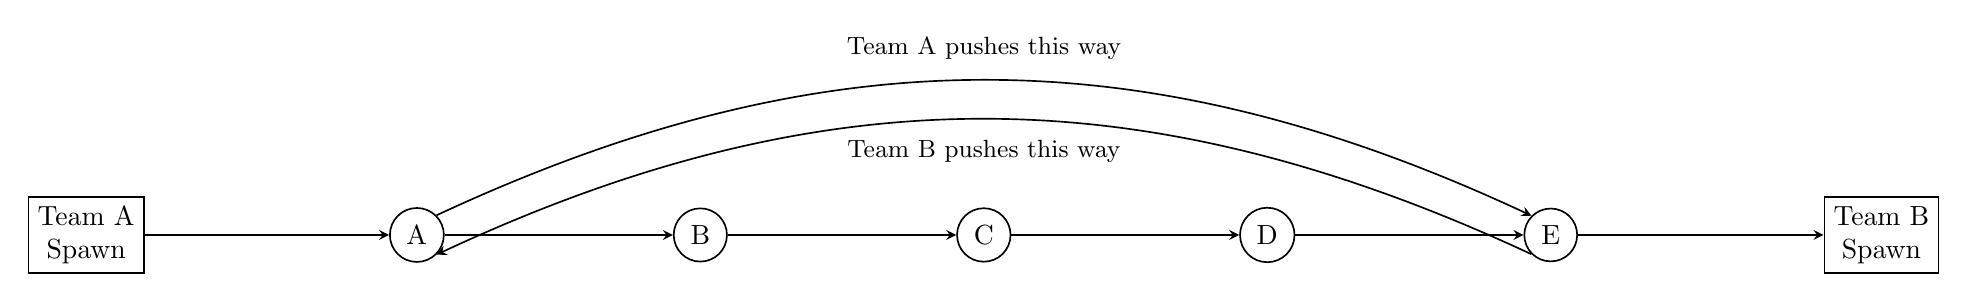
\begin{tikzpicture}[node distance=2cm, ->, >=stealth, semithick]

    % Define nodes
    \node (Aspawn) [draw, rectangle, minimum width=1.3cm, align=center] {Team A\\Spawn};
    \node (Apoint) [draw, circle, right of=Aspawn, xshift=2.2cm] {A};
    \node (Bpoint) [draw, circle, right of=Apoint, xshift=1.6cm] {B};
    \node (Cpoint) [draw, circle, right of=Bpoint, xshift=1.6cm] {C};
    \node (Dpoint) [draw, circle, right of=Cpoint, xshift=1.6cm] {D};
    \node (Epoint) [draw, circle, right of=Dpoint, xshift=1.6cm] {E};
    \node (Bspawn) [draw, rectangle, minimum width=1.3cm, align=center, right of=Epoint, xshift=2.2cm] {Team B\\Spawn};

    % Straight connections for the 'linear' look
    \draw[->] (Aspawn) -- (Apoint);
    \draw[->] (Apoint) -- (Bpoint);
    \draw[->] (Bpoint) -- (Cpoint);
    \draw[->] (Cpoint) -- (Dpoint);
    \draw[->] (Dpoint) -- (Epoint);
    \draw[->] (Epoint) -- (Bspawn);

    % Larger bends and position tweaks for clarity
    \draw[->, bend left=25] (Apoint.north east) 
        to node[pos=0.5, above, yshift=4pt, align=center]{\small Team A pushes this way}
        (Epoint.north west);

    \draw[->, bend right=25] (Epoint.south west) 
        to node[pos=0.5, below, yshift=-4pt, align=center]{\small Team B pushes this way}
        (Apoint.south east);

\end{tikzpicture}
}%
\caption{Linear layout of Clash objectives and spawns,}
\label{fig:clash-layout}
\end{figure}

As shown in Figure \ref{fig:clash-layout}, Team A is associated with point A 
and Team B with point E. Once the game designates who is defending or attacking 
each side, that \emph{role remains} regardless of score changes.

\section{Implications for Gameplay}
\subsection{Prolonged Stalemates}
If a team fights back from a deficit, the defenders retain a home-field advantage 
that can lead to lengthy standoffs. Even when the score is effectively even, 
the nominal ``defender'' has a short reinforcement route.

\subsection{Snowball Potential}
Alternatively, if the ``attacking'' team quickly wins early fights, they may chain 
captures before the defenders stabilize. This can feel like an unstoppable push 
due to respawn timers lining up poorly for the losing team.

\section{Potential Solutions}

\subsection{Dynamic Role Reassignment}
Reevaluate spawns upon a tie (e.g., 4--4). Move both spawns to a neutral midpoint 
or define symmetrical spawns so neither side has a perpetual advantage.

\subsection{Adaptive Spawn Shifts}
Allow spawn points to shift incrementally based on live conditions. For instance, 
if the enemy retakes a lost objective, the original defenders do not keep the 
previous spawn advantage.

\subsection{Layout Redesign}
Consider redesigning final objectives so each side’s spawn advantage is tempered. 
For instance, allow more flanking routes that attackers can use, or ensure defenders 
cannot quickly recontest without a penalty.

\section{Conclusion}
Clash mode demonstrates a creative attempt to merge elements of Assault and Control. 
However, the locked-in roles for attackers and defenders can create persistent 
spawn advantages that do not reflect the real-time match state. Addressing this 
issue may require spawn logic revisions or a more fundamental map layout change. 
Revisiting the mode’s design is essential to ensure fair competition and preserve 
Overwatch 2’s fast-paced, teamwork-centric gameplay.

\appendix
\section{References}
\begin{enumerate}
    \item Developer Update: Hero Releases, Mythics, and Gameplay Updates. Blizzard 
    Entertainment, March 19, 2024.
    \item Season 12: New Frontiers Official Trailer | Overwatch 2. PlayOverwatch, Aug 14, 2024.
    \item Overwatch 2 Patch Notes, various 2024 updates. Blizzard Entertainment.
    \item Community discussions on Overwatch forums and Reddit regarding Clash spawn 
    issues. 
\end{enumerate}

\end{document}
